\documentclass{article}
\usepackage[utf8]{inputenc}
\usepackage{authblk}
\usepackage{setspace}
\usepackage[margin=1.25in]{geometry}
\usepackage{graphicx}
\graphicspath{ {./figures/} }
\usepackage{subcaption}
\usepackage{amsmath}
\usepackage{lineno}
\usepackage{xcolor}
\usepackage{multirow}
\linenumbers

%%%%%% Bibliography %%%%%%
% Replace "sample" in the \addbibresource line below with the name of your .bib file.
\usepackage[style=ieee,
citestyle=numeric-comp,
sorting=none]{biblatex}
\addbibresource{reference.bib}

%%%%%% Title %%%%%%
% Full titles can be a maximum of 200 characters, including spaces.
% Title Format: Use title case, capitalizing the first letter of each word, except for certain small words, such as articles and short prepositions
\title{Learning Rat-Like Behavioral Interaction Using a Small-Scale Robotic Rat}

%%%%%% Authors %%%%%%
% Authors should be listed in order of contribution to the paper, by first name, then middle initial (if any), followed by last name.
% Authors should be listed in the order in which they will appear in the published version if the manuscript is accepted.
% Use an asterisk (*) to identify the corresponding author, and be sure to include that person’s e-mail address. Use symbols (in this order: †, ‡, §, ||, ¶, #, ††, ‡‡, etc.) for author notes, such as present addresses, “These authors contributed equally to this work” notations, and similar information.
% You can include group authors, but please include a list of the actual authors (the group members) in the Supplementary Materials.
\author[1,2$\dag$]{Hongzhao Xie}
\author[1,2$\dag$]{Zihang Gao}
% \author[2]{Author Three}
% \author[1,2]{Author Four}

%%%%%% Affiliations %%%%%%
\affil[1]{Intelligent Robotics Institute, School of Mechatronical Engineering, Beijing Institute of Technology, Beijing 100081, China}
\affil[2]{Key Laboratory of Biomimetic Robots and Systems (Beijing Institute of Technology), Ministry of Education, Beijing 100081, China}

%%%%%% Date %%%%%%
% Date is optional
\date{}

%%%%%% Spacing %%%%%%
% Use paragraph spacing of 1.5 or 2 (for double spacing, use command \doublespacing)
\onehalfspacing

\begin{document}

\maketitle

%%%%%% Abstract %%%%%%
\begin{abstract}
In the existing robot-rat interaction, robots usually exert influence as stimuli to observe the response of target rats. However, the above single-stimulation model from robot to rat lacks a two-way communication. Therefore, we proposed a method to learn the rat-like behavioral interaction. First, we constructed two behavior patterns in the interaction process between the two rats: the individual pattern and the interaction pattern. We divided the roles of the two rats into active stimulator and passive receiver. The stimulator executes the individual pattern, and the receiver switches between the two patterns. Which pattern the receiver executes depends on the probability of interaction. Secondly, we proposed a hypothesis concerning the behavioral interaction between two rats and controlled the interaction process between two robots. Information entropy was used to measure the similarity between two robots and two rats. The results proved that the probability of interaction between rats depends on the distance of centroid and average relative velocity, and we obtained the optimal solution to express the relationship between them. In the future, the improvement of robots' interaction ability with rats will highly benefit from this study.
\end{abstract}

%%%%%% Main Text %%%%%%
\section{Introduction}
In recent years, due to the progress of robot technology and the reduction in cost, biomimetic robots have been increasingly used in animal behavior research. Biomimetic robots are easier to operate than real animals, and their behavior characteristics can be accurately controlled \cite{abdai_poking_the_futhre, yeager_new_tech}. Through effective control methods and active guidance, these robots can interact with animals, observe and record their reactions \cite{son_entice_insect,Taylor2008frogs-17969,kopman_closed_loop_zebrafish,partan_wild_tree,5650930}. Sometimes, biomimetic robots are placed in a group of animals to explore their behavior mechanism, or to verify scientific assumptions in the process of interaction \cite{doi:10.1126science.1144259,ward_quorum,gribovskiy_mobile_robot,faria_novel_method}. For example, Kopman \textit{et al.} studied the response of zebrafish to a robotic fish. The robotic fish is similar to the real zebrafish in shape and color. The experimental results show that the the response of zebrafish changes with the tail-beating pattern of the robotic fish \cite{kopman_closed_loop_zebrafish}. Halloy \textit{et al.} introduced a specially designed biomimetic autonomous robot into cockroaches to study the collective decision-making behavior of cockroaches in shelter selection \cite{doi:10.1126science.1144259}.

The social activities of rats have attracted the interest of many researchers, and these studies have achieved remarkable results \cite{fleliz_bidirectional_modulation,weiss_shall_two_walk}. Because of the advantages of biomimetic robots in animal interactions, various rat-like robots have been designed for the study of rats \cite{Lucas2018DesignOA,Shi_bb_2013,Shi_bb_2015,shi-gao-tro-2022}. Ortiz \textit{et al.} designed a robotic rat (e-puck) with a simple behavior pattern to explore whether the robot can interact well with actual rats and trigger their social behaviors \cite{Rusalky-sit}. Heath et al. developed a biomimetic robotic rat (Pirat), which is similar in size to the real rat. The influence of the robot on rat behaviors was tested by controlling different behaviors of the robot (frequent approach and avoidance) \cite{pirat}. Sullivan \textit{et al.} designed a robot imitating the behavior of rat pups, and planned the input/output cognitive architecture for the robot through a genetic algorithm to deeply understand the behavior of Norwegian rat pups \cite{sullivan-arl-2015}. However, these robots have fewer degrees of freedom (DOFs) and lack flexibility in local motion, so it is difficult to simulate the complex and diverse behavior patterns of rats. In addition, the current research on robot-rat interaction usually adopts the method of directly controlling the movement and behavior of the robot. The robot acts as a stimulus to exert influence to observe the response of the target rat. There are few studies on the behavioral interaction between rats. We believe that learning the behavioral interaction of rats is indeed a means to promote the effect of robot-rat interaction.

In this paper, we first constructed two behavior patterns of rat interaction: the individual pattern and the interaction pattern. In our previous study, we learned the individual behavior law of rats in the open field and applied it to a small-scale robotic rat platform \cite{gao-eng-2022}. The robot has 4 DOFs in the pitch direction and 3 DOFs in the yaw direction. It can perform movements and behaviors similar to those of rats with a high degree of flexibility \cite{shi-gao-tro-2021}. Therefore, we used the previously obtained behavior law to build the individual pattern of rats.

Relatively, the interaction pattern of rats can be divided into different states, such as tracking and imitating. The two rats participating in the interaction process usually show different roles, one is the active stimulator and the other is the passive receiver. The behavior of the receiver is determined by the stimulator. When learning the behavioral interaction of rats, a difficult problem is that the roles played by a rat usually change with each other. That is, the same rat may be both a stimulator and a receiver at different times, and it depends on the characteristics of the individual. Hence, we proposed the following strategy: not distinguish the individual of rats, but only distinguish the stimulator and receiver. The stimulator executes the individual pattern, and the receiver switches between the individual pattern and the interaction pattern. Which pattern the receiver executes depends on the probability of interaction.

Furthermore, we learned the rat-like behavioral interaction by controlling the interaction process of the two robots. The similarity of behavioral interaction between robots and rats is measured by interaction information entropy. A hypothesis concerning the behavioral interaction of rats is proposed; that is, the probability of interaction between rats depends on the distance of the centroid and the average relative velocity. According to the results of robot interaction control and hypothesis test, we proved the rationality of the above hypothesis, and obtained the optimal solution expressing their relationship. Figure \ref{process-of-robot-learn} presents the process of robot learning rat-like behavioral interaction. Robots learn similar behavior patterns and the interaction process form rats to realize a more natural and effective robot-rat interaction. This is of great significance to future robot-rat interactions.

\begin{figure}[h]
    \centering
    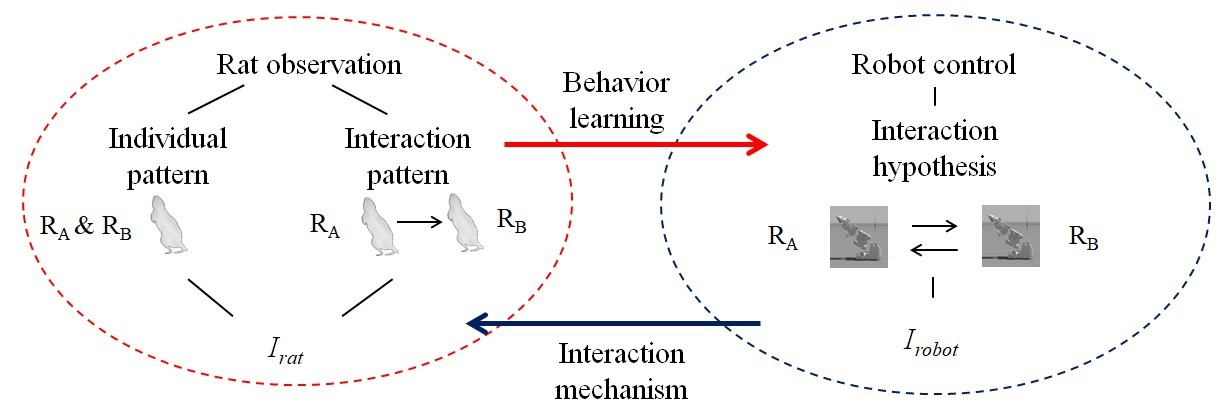
\includegraphics[width=0.8\textwidth]{process-of-robot-learn}
    \caption{The process of robot learning rat-like behavioral interaction.}
    \label{process-of-robot-learn}
\end{figure}

\section{Two Behavior Patterns of Interaction}
\subsection{Individual Pattern}
The open-field test is used to study the spontaneous activities of animals in a
new environment. It allows experimental animals to move freely in a certain
space with few restrictions, and has become an important method to study animal
movements and behaviors \cite{PRUT20033, EILAM200353}. Scientists usually divide
the movements of rats into movements such as going straight, turning, standing
up, and staying in one place. Correspondingly, the behaviors of rats are divided
into behaviors such as exploring, grooming, and resting to reflect the different
activity characteristics of rats\cite{the_rat_study,whishow_bejavior,
MARSHALL2021420,dunn_profiling}. In this paper, we observed the activities of
individual rats (Rattus norvegicus) in a $1{\rm m}\times 1{\rm m}\times 1{\rm m}
$ open field, and marked the key movement joints of rats. Through the records of
10 min a day, we obtained a dataset of the movements of three rats over five
days. The rats involved in this study came from the same litter and were seven
weeks old. The dataset (150 min) contains 3537 rat movements.

Through the observation of rat data, we found that there were some specific
combinations in the movement time series of rats. The frequency of these
combinations is relatively high, which can reflect the activity characteristics
of rats. Therefore, we used a softmax classifier to map the combination of
movements to the behavior, and counted the probability distribution of the
combinations and behaviors. Table \ref{table:movement and behavior of rats} 1
shows the movement and behavior of the rats we observed.
Table \ref{table:relevancy between each movement combination and behavior} shows
the relevancy between each movement combination and behavior (the numbers in
brackets represent the probability). We built the individual pattern of rats on
the basis of the behavior law shown in Table
\ref{table:relevancy between each movement combination and behavior}.
% \begin{table}[b]
%     \caption{Movement and Behavior of Rats}
%     \centering
%     \begin{tabular}{cccc}
%             \hline
%             Movement & Symbol & Behavior & Symbol \\
%             \hline
%             Head pitching & $M_1$ & Sniffing & $B_1$ \\
%             Head yawing & $M_2$ & Exploring & $B_2$ \\
%             Body pitching & $M_3$ & Walking & $B_3$ \\
%             Body yawing & $M_4$ & Trotting & $B_4$ \\
%             Going Straight & $M_5$ & Resting & $B_5$ \\
%             Turning & $M_6$ & Grooming & $B_6$ \\
%             Staying & $M_7$ & & \\
%             Forelimb swing & $M_8$ & & \\
%             \hline
%             \end{tabular}
%     \label{table:movement and behavior of rats}
% \end{table}

\begin{table}[b]
    \caption{Relevancy Between Each Movement Combination and Behavior}
    \centering
    \begin{tabular}{cc}
            \hline
            Movement combination & Behavior \\
            \hline
            Head pitching & $M_1$ \\
            Head yawing & $M_2$ \\
            \hline
            \end{tabular}
    \label{table:relevancy between each movement combination and behavior}
\end{table}

\subsection{Interaction Pattern}
The interaction between rats will appear in various states, such as tracking,
imitating and contacting. At present, there are still great difficulties in
contact simulation of the robot (insufficient freedom of forelimbs, difficult to
accurately control contact parts and contact forces, etc.). Hence, we avoid
contacting when controlling the robot interaction. When counting the rat
behavior data, the probability of rat contacting is transformed into tracking
and imitating in proportion.

To effectively learn the interactive behavior model between rats, we defined A
as the rat that actively generates the interaction intention and B as the rat
that passively responds to the interaction. Among them, the stimulator (${\rm
R_A}$) executes the individual pattern, and the receiver (${\rm R_B}$) switches
between the individual pattern and the interaction pattern. In the interaction
pattern, the behavior of ${\rm R_B}$ is determined by ${\rm R_A}$. Which pattern
${\rm R_B}$ executes depends on the probability of interaction ($\rm
P_{interaction}$) between two rats, as show in Figure \ref{interaction-process}.
$a_{i+1}$, $b_i$ and $b_{i+1}$ are the behavior of ${\rm R_A}$ at $t_{i+1}$,
${\rm R_B}$ at $t_i$ and ${\rm R_B}$ at $t_{i+1}$ respectively.
\begin{figure}[h]
    \centering
    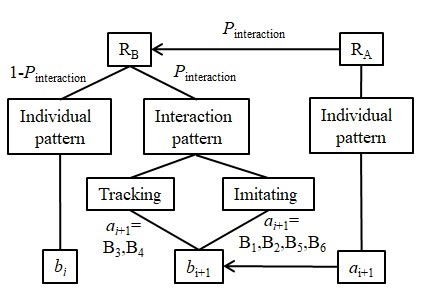
\includegraphics[width=0.8\textwidth]{interaction-process.jpg}
    \caption{The interaction process between $\rm R_A$ and $\rm R_B$.}
    \label{interaction-process}
\end{figure}
Furthermore, we verified the rationality of the proposed strategy. We observed
the interaction process between the rats. We divided three rats, 1, 2 and 3,
into three groups and placed them in a $1{\rm m}\times 1{\rm m}\times 1{\rm m}$
open field in pairs (rats 1 and 2; rats 1 and 3; rats 2 ant 3). Each group
recorded 20-min rat behavior data. During the recording process, the active rat
is always marked as A and the passive rat is marked as B. Then, we obtained
approximately 1000 behavior data of rats A and B, respectively. We counted the
behavior probability distribution of rats A and B in the process of interaction,
and the joint hypotheses test (F-test) was used to verify whether the behavior
probability distribution of rats in the interaction was consistent with that in
the individual pattern. Our results are shown in Table \ref{table:Behavior
Probability Distribution of Rats}. It can be seen that there is no significant
difference between the behavior distribution probability of $\rm R_A$ and that
of individuals, that is, $\rm R_A$ always executes the individual pattern; the
behavior distribution probability of RB is significantly different from that of
individuals, so the behavior of $\rm R_B$ is affected by $\rm R_A$.
\begin{table}[b]
    \caption{Behavior Probability Distribution of Rats}
    \centering
    \begin{tabular}{cccc}
            \hline
            Behavior & Individual & $\rm R_A$ & $\rm R_B$ \\
            \hline
            $\rm B_1$ & 0.015 & 0.05 & 0.1 \\
            $\rm B_2$ & 0.284 & 0.15 & 0.05 \\
            $\rm B_3$ & 0.16 & 0.35 & 0.5 \\
            $\rm B_4$ & 0.167 & 0.15 & 0.05 \\
            $\rm B_5$ & 0.213 & 0.15 & 0.1 \\
            $\rm B_6$ & 0.071 & 0.15 & 0.2 \\
             &  & ${\rm F}=1.67<{\rm F}_{0.05,(5,5)}=5.05$ & ${\rm F}=5.13<{\rm F}_{0.05,(5,5)}=5.05$ \\
            \hline
            \end{tabular}
    \label{table:Behavior Probability Distribution of Rats}
\end{table}

\section{Rat-Like Behavior Interaction}
\subsection{Robotic Rat Platform}
The prototype of our recently developed robotic rat is shown in Figure
\ref{figure:robot-system}. The robot is mainly composed of the head, forelimb,
waist and hip. The head and hip joints are driven by servo motors, the waist
joints and wheels are driven by DC motors, and the forelimb is driven by a micro
deceleration stepper motor. Its shape and size are similar to those of actual
rats, with a total mass of approximately 400 g. The spinal joints of the robot
correspond to the key movement joints of rats. The head pitching and yaw
movements ($M_1, M_2$) are performed by $J_7$ and $J_6$ respectively; the body
pitching movement $M_3$ is performed by $J_1$, $J_2$ and $J_5$; the body yaw
movement ($M_4$) is performed by $J_3$ and $J_4$; the straight movement ($M_5$)
is performed by the driving wheels ($J_{WL}$, $J_{WR}$); the turing movement
($M_6$) is performed by the yaw joints compound driving wheels ($J_3$, $J_4$,
$J_6$, $J_{WL}$, $J_{WR}$); and the forelimb swing movement ($M_8$) is performed
by $J_F$.

\begin{figure}[h]
    \centering
    \begin{subfigure}{0.4\textwidth}
        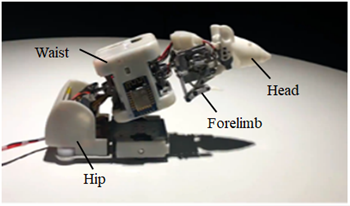
\includegraphics[height=1.3in]{roboticrat.png}
        \caption{\label{figure:roboticrat}}
    \end{subfigure}
    \begin{subfigure}{0.5\textwidth}
        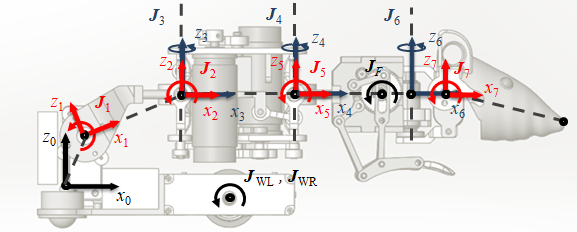
\includegraphics[height=1.3in]{coord.png}
        \caption{\label{figure:motion-coord}}
    \end{subfigure}
    \caption{(\subref{figure:roboticrat}) Robotic rat. (\subref{figure:
    motion-coord}) Motion coordinate system of the robotic rat.}
    \label{figure:robot-system}
\end{figure}

To make the robot achieve the above behaviors, we extracted the characteristic
parameters for each movement combination, as shown in Table \ref{table:Movement
Parameters}. These parameters determine the amplitude, average speed, frequency
and duration of rat movements. In our previous work, we proved that the robot
can complete the movement of rats with a high biomimicry degree, and the
trajectory of each joint of the robot can be expressed by the above
characteristic parameters \cite{shi-gao-tro-2021}. Here, to adapt to the
diversity of rat movement parameters, we first used cluster analysis to extract
the dominant values of these characteristic parameters
\cite{fraley_how_many_clusters,kaufman_finding_groups}. Furthermore, a
two-hidden-layer BP neural network is used to learn and generate the trajectory
of each joint of the robot, as shown in Figure. \ref{figure:Joint Trajectory
learning by a two hidden-layer BP neural network}. The tanh activation function
is used to accelerate the convergence of the network
\cite{inohira-generalization}. $\theta_1-theta_7$ represent the angular
displacement of robot spine joints, $\theta_f$ represents the angular
displacement of robot forelimb joint, and $\omega_l,~\omega_r$ represent the
angular velocity of robot driving wheels.

\begin{table}[b]
    \caption{Movement Parameters}
    \centering
    \begin{tabular}{cc}
            \hline
            Movement parameters & Symbol \\
            \hline
            Head pitch angle & $\phi_{hp}$ \\
            Head yaw angle & $\phi_{hy}$ \\
            Body pitch angle & $\phi_{bp}$ \\
            Body yaw angle & $\phi_{by}$ \\
            Forelimb swing angle & $\phi_{fs}$ \\
            Turning angle & $\alpha$ \\
            Average forward speed & $\nu$ \\
            Movement frequency & $f$ \\
            Movement duration & $f$ \\
            \hline
            \end{tabular}
    \label{table:Movement Parameters}
\end{table}

\begin{figure}[h]
    \centering
    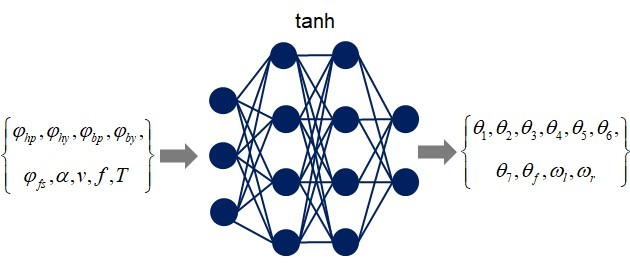
\includegraphics[width=0.8\textwidth]{network.jpg}
    \caption{Joint Trajectory learning by a two hidden-layer BP neural network.}
    \label{figure:Joint Trajectory learning by a two hidden-layer BP neural
    network}
\end{figure}

\subsection{Interaction Hypothesis}
Based on our robotic rat platform, we hope to learn the rat-like behavioral
interaction by controlling the interaction process between two robots. Therefore,
we put forward the following hypothesis: The interaction probability
$P_{interaction}$ is affected by the centroid distance ($d_m$) and the average
relative speed ($\nu_m$) between $\rm R_A$ and $\rm R_B$. We assumed that the
smaller the centroid distance, or the larger the average relative speed between
$\rm R_A$ and $\rm R_B$, the greater the probability of $\rm R_B$ executing the
interaction pattern, as shown in the following formula:
\begin{equation} \label{eq:probability of interaciton}
    \displaystyle\begin{cases}
        u=\displaystyle\frac{\nu/V_m}{d_m/D_m} \\
        P_{interaciton}(u)=\displaystyle\frac{p_{+\infty}-p_{-\infty}}{1+e^{-ku}}
        +p_{-\infty}
    \end{cases}
\end{equation}

where $V_m$ and $D_m$ are the maximum values of average relative speed and
centroid distance between $\rm R_A$ and $\rm R_B$, respectively, $-1\leq
v_m/V_m\leq 1$ (the inner side of the centroid line is positive and the outer
side is negative), $0\leq d_m/D_m\leq 1$ ($d_m>0$, because the defined
interaciton process is noncontact). $p_{+\infty},p_{-\infty}$ and $k$ are
interaction coefficients, which represent the lower limit, upper limit and scale
factor of interaction probability $P_{interaciton}$, respectively, as shown in
Figure. \ref{figure:relationship between the interaciton probability and
independent variable}.
\begin{figure}[h]
    \centering
    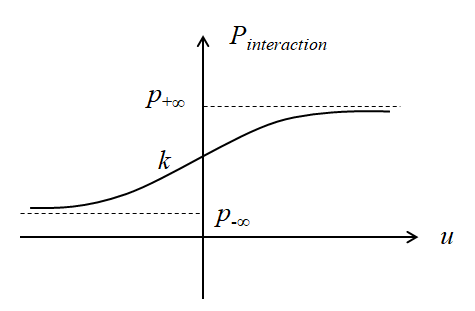
\includegraphics[width=0.8\textwidth]{interaction-probability.png}
    \caption{Relationship between the interaciton probability $P_{interaction}$
    and independent variable $u$.}
    \label{figure:relationship between the interaciton probability and
    independent variable}
\end{figure}

In this paper, we used interaction information entropy to measure the
interaction similarity between robots and rats \cite{lellis-feedback-control},
as shown in the following formula:
\begin{equation} \label{eq:interaction similarity}
    I(R_A,R_B)=\sum_{a_{i+1},b_i,b_{i+1}}p(a_{i+1},b_i,b_{i+1})\log_{2}
    \frac{p(b_{i+1}|a_{i+1}),b_{i}}{b_{i+1}|b_i}
\end{equation}
where $\rm R_A$ and $\rm R_B$ are the two rats or two robots that produce
interaction. $I$ represents the amount of interaction information between two
rats or two robots. The closer the amount of interaction information of robots
is to the actual rats, the closer the interaction process of the two is.
\textcolor{red}{$\Delta t~(t_i\rightarrow t_{i+1})$ is the movement duration
$T_A$ of $\rm R_A$.}

\subsection{Robot Interactive Control}
In the interaction pattern, when $\rm R_A$ shows walking or trotting behavior,
the state of $\rm R_B$ is tracking; when $\rm R_A$ shows other behaviors, the
state of $\rm R_B$ is imitating. For the imitating state, the movement
parameters of $\rm R_B$ are equal to those of $|rm R_A$. For the tracking state,
as shown in Figure. \ref{figure:movement parameters of RB in the tracking state}
. when the movement parameters of $\rm R_A$ are known, the movement parameters
of $\rm R_B$ are as follows:
\begin{equation} \label{eq:movement parameters}
    \begin{cases}
        \nu_B=d_{m'}/T_A \\
        \alpha_B=\beta - \delta \\
        T_B=T_A
    \end{cases}
\end{equation}
\begin{figure}[h]
    \centering
    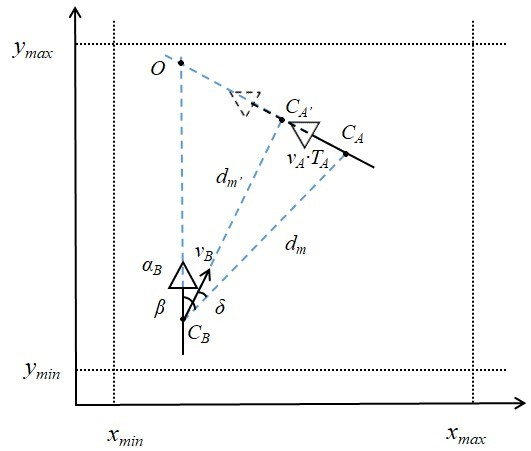
\includegraphics[width=0.8\textwidth]{movement parameters of rb.jpg}
    \caption{Movement parameters of $\rm R_B$ in the tracking state.}
    \label{figure:movement parameters of RB in the tracking state}
\end{figure}
$C_A,~C_{A'}$ and $C_B$ are the centroids of $\rm R_A$ at $t_i$ and $t_{i+1}$,
and $\rm R_B$ at $t_{i+1}$ respectively.

In addition, we considered the problem of robot collision avoidance, as shown in
Figure. \ref{figure:obstacle avoidance analysis}. Figure. \ref{figure:obstacle
avoidance analysis}-\ref{figure:Avoid collision with boundary} shows the process
of the robot avoiding collision with the boundary (wall). The condition of
obstacle avoidance and the configuration of robot movement parameters are shown
in Equation (\ref{eq:configuration of robot movement parameters}). Figure.
\ref{figure:obstacle avoidance analysis}-\ref{figure:Avoid collision between
robots} shows the process of avoiding collisions between robots. The condition
for obstacle avoidance and the configuration of robot movement parameters are
shown in Equation (\ref{eq:configuration2 of robot movement parameters}).

\begin{figure}[h]
    \centering
    \begin{subfigure}{0.4\textwidth}
        \centering
        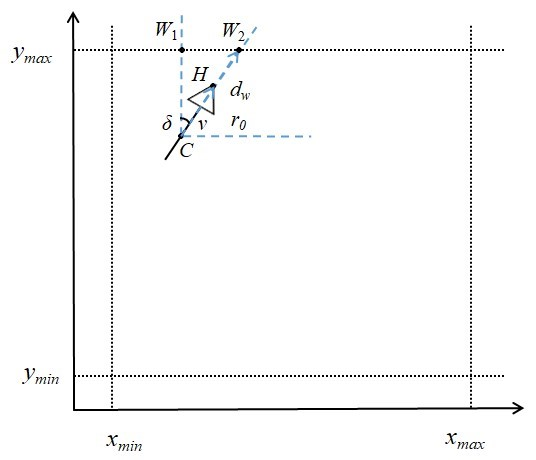
\includegraphics[height=2.2in]{collision-avoidance.jpg}
        \caption{\label{figure:Avoid collision with boundary}}
    \end{subfigure}
    \begin{subfigure}{0.4\textwidth}
        \centering
        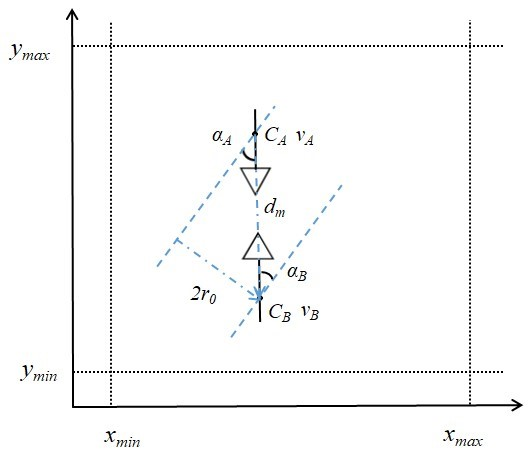
\includegraphics[height=2.2in]{collision-avoidance-between-robots.jpg}
        \caption{\label{figure:Avoid collision between robots}}
    \end{subfigure}
    \caption{Obstacle avoidance analysis. (\subref{figure:roboticrat}) Avoid
    collision with boundary (wall); (\subref{figure:motion-coord}) Avoid
    collision between robots.}
    \label{figure:obstacle avoidance analysis}
\end{figure}
\begin{equation}\label{eq:configuration of robot movement parameters}
    \begin{cases}
        d_w\leq D_w^{avoid} \\
        D_w^{avoid} = T_{control}\cdot \nu +r_0 \\
        \nu \rightarrow 0, \alpha=\pi/2-\delta, T_{control}
    \end{cases}
\end{equation}
\begin{equation}\label{eq:configuration2 of robot movement parameters}
    \begin{cases}
        d_m\leq D_m^{avoid} \\
        D_m^{avoid} = T_{control}\cdot \nu_m + 2r_0 \\
        \nu_A \rightarrow 0, \alpha_A, T_{control} \\
        \nu_B \rightarrow 0, \alpha_B, T_{control}
    \end{cases}
\end{equation}

\subsection{Hypothesis Test}
First, we observed the interaction process and calculated the interaction
information entropy between rats ($I_{rat}=1.207$). Then, we gave a series of
values of $p_{-\infty}, p_{+\infty}$ and $k$, and calculated the value of
$I_{robot}$ in the interaciton time $T_{interaciton}$. $T_{interaciton}$ is the
shortest time to make the interaction process converge. When the behavior
probability distribution of the robot tends to be stable, we believe that the
interaction process converges. Our results are shown in Table \ref{table:INTERACTION INFORMATION ENTROPY OF ROBOTS}.
\begin{table}[b]
    \caption{Interaction Information Entropy of Robots}
    \centering
    \begin{tabular}{ccccc}
            \hline
            $p_{-\infty}$ & $p_{+\infty}$ & $k$ & $I_{robot}$ & $\hat{I}_{robot}$\\
            \hline
            0.2 & 0.4 & 0.5 & 0.8987 & 0.9541 \\
            0.3 & 0.5 & 1 & 1.156 & 1.091 \\
            0.4 & 0.6 & 1.5 & 1.256 & 1.228 \\
            0.5 & 0.7 & 2 & 1.337 & 1.365 \\
            0.6 & 0.8 & 2.5 & 1.494 & 1.502 \\
            \hline
            \end{tabular}
    \label{table:INTERACTION INFORMATION ENTROPY OF ROBOTS}
\end{table}

After data analysis, we found that the independent variables have a significant
impact on the dependent variable with a close linear correlation. Therefore, we
used a multiple linear regression model to fit the relationship between
independent variables and dependent variables, as shown in Equation (\ref{eq:
multiple linear regression model}).
\begin{equation}\label{eq:multiple linear regression model}
    \hat{I}_{robot}=a_0+a_1p_{-\infty}+a_2p_{+\infty}+a_3k
\end{equation}
where the coefficients $a_i, i=0,1,2,3$ are calculated as follows ($n$ is the number of samples).
\begin{equation*}
    \left[\begin{array}{c}
        a_0 \\
        a_1 \\
        a_2 \\
        a_3 \\
    \end{array}\right]=\left[\begin{array}{cccc}
        n & \sum p_{-\infty} & \sum p_{+\infty}  & \sum k \\
        \sum p_{-\infty} & \sum p^2_{-\infty} & \sum p_{-\infty}p_{+\infty}  &
        \sum p_{-\infty} k \\
        \sum p_{+\infty} & \sum p_{-\infty} p_{+\infty} & \sum p^2_{+\infty}  &
        \sum p_{+\infty} k \\
        \sum k & \sum p_{-\infty} k & \sum p_{+\infty} k  & \sum k^2 \\
    \end{array}\right]^{-1}
    \left[\begin{array}{c}
        \sum I_{robot} \\
        \sum p_{-\infty} I_{robot} \\
        \sum p_{+\infty} I_{robot} \\
        \sum kI_{robot} \\
    \end{array}\right]
\end{equation*}
After calculation, we obtained $a_0=1.7282, a_1=0.1128, a_2=0.2584$, and $
a_3=0.0119$.

Furthermore, we obtained a set of control variables through parameter
optimization, which makes the interaction information entropy of two robots and
two rats closest. The Equation shows the process of parameter optimization, and
the optimal solution is
\begin{equation}
    \begin{cases}
        p_{-\infty},p_{+\infty},k=\arg\min f \\
        \min f(p_{-\infty},p_{+\infty},k)=\displaystyle\frac{|I_{robot}-I_{rat}|}
        {I_{rat}} \\
        s.t.~0<p_{-\infty}<p_{+\infty}<1 \\
    \end{cases}
\end{equation}

We calculated the interaction information entropy between robots (10 times) by
the optimal solution of control variables, and the results are shown in Table
\ref{table:INTERACTION INFORMATION ENTROPY OF ROBOTS AND RATS}. The t-test shows
that there is no significant difference between the interaction information
entropy of two robots and two rats; that is, our hypothesis has been verified.
\begin{table}[b]
    \caption{Interaction Information Entropy of Robots and Rats}
    \centering
    \begin{tabular}{ccc}
            \hline
            $I_{robot}$ & ${I}_{rat}$ & t-test \\
            \hline
            1.210 &\multirow{9}{*}{1.207} & \multirow{9}{*}{$\begin{array}{l}
                H_0:\bar{I}_{robot}=I_{rat}; \\ H_1:\bar{I}_{robot}\neq I_{rat};
                \\ t=1.583<t_{0.025,9}=2.262
            \end{array}$} \\
            1.108 & & \\
            1.208 & & \\
            1.206 & & \\
            1.207 & & \\
            1.211 & & \\
            1.207 & & \\
            1.205 & & \\
            1.205 & & \\
            \hline
            \end{tabular}
    \label{table:INTERACTION INFORMATION ENTROPY OF ROBOTS AND RATS}
\end{table}

\section{Discussion}
This paper aims to learn the behavioral interaction of rats through the control of robotic rats. We proposed two behavior patterns in the interaction process of rats and the hypothesis of the behavioral interaction. After testing, we proved that the interaction probability between rats depends on the distance of the centroid and the average relative velocity, and obtained the optimal solution expressing their relationship. The robots learn similar movements and behaviors from rats, and then understand the interactive behavior mechanism of rats, which can significantly help us realize a more natural and effective robot-rat interaction process.

The deficiency of this study is that in the interactive control of robots, the contacting state is not considered. In future work, we will plan to simulate the contacting state of rats by increasing the DOFs of robots' forelimbs and nesting rat skins to make the robot closer to the real rats.
In this study, the rat that actively generates interaction intention is recorded as A, and the rat that passively interacts is recorded as B. In the future robot-rat interaction process, the proportion of active interaction intention (behavior) of the robot can be adjusted to play different roles (lively/quiet, strong/weak). After understanding the personality characteristics of the interaction target, the robot can make corresponding adjustments to adapt to different rat individuals to produce a better interaction effect.

This study only explored the effects of visual factors on rat interactive behavior, including centroid distance and average relative velocity. In future studies, we can add sound (ultrasound, which can reflect the emotional state of rats), smell and other factors, and give these characteristics to the robot to explore the interaction process of rats at other levels.


% %%%%% Citations in the text %%%%%%
% \subsection*{Citations}
% % Citations of references in the text should be identified using numbers in square brackets e.g., ``as discussed by Cui \cite{Cui1}'' or ``as discussed elsewhere \cite{Cui1,Ninomiya1,Li1,Wang1,Yang1}.'' All references should be cited within the text and uncited references will be removed.

% As an example, this template includes a ``sample.bib'' file containing the references in BibTeX.

% %%%%%% Equations %%%%%%
% \subsection*{Equations}
% Equations should be provided in a text format, rather than as an image. Equations should be numbered consecutively, in round brackets, on the right-hand side of the page by using the ``\textbackslash begin\{equation\}'' command. They should be referred to as Equation 1, etc. in the main text.

% \medskip For example, see Equation \ref{eq:1} and Equation \ref{eq:2} below.
% \begin{equation} \label{eq:1}
%     a^2 + b^2 = c^2
% \end{equation}
% \begin{equation} \label{eq:2}
% \begin{split}
% A & = \frac{\pi r^2}{2} \\
%  & = \frac{1}{2} \pi r^2
% \end{split}
% \end{equation}

% %%%%%% Figures %%%%%%
% \subsection*{Figures}
% Figures should be called out within the text and numbered in the order of their citation in the text. Every figure must have a descriptive title beginning with ``Figure [Number] …'' All figure titles should be either a phrase or a sentence; do not mix the two styles. See Figure \ref{fig:1} for example.
% \begin{figure}[h]
%     \centering
%     
\includegraphics[width=0.5\textwidth]{fig 1}
%     \caption{This is an example figure.}
%     \label{fig:1}
% \end{figure}

% Figures should be displayed on a white background. When preparing figures, consider that they can occupy either a single column (half page width) or two columns (full page width), and should be sized accordingly.

% If a figure consists of multiple panels, they should be ordered logically and labelled with lower case roman letters (i.e., a, b, c, etc.). All labels should be explained in the legend. See Figure \ref{fig:2} for example.

% Upon acceptance, authors will be asked to provide the figures as separate electronic files. At that stage, figures should be supplied in either vector art formats (PS, EPS, FIG, AI, Visio, WMF, EMF, Word, Excel, PowerPoint, OPJ, CDR, or PDF) or bitmap formats (Photoshop, TIFF, GIF, JPEG, PNG, BMP, etc.). Bitmap (BMP) images should be of at least 300 dpi resolution, unless due to the limited resolution of a scientific instrument. If a bitmap image has labels, the image and labels should be embedded in separate layers.
% \begin{figure}[h]
%     \centering
%     \begin{subfigure}{0.4\textwidth}
%         
\includegraphics[width=0.9\textwidth, height=2in]{fig 1}
%         \caption{\label{fig:2a}}
%     \end{subfigure}
%     \begin{subfigure}{0.4\textwidth}
%         
\includegraphics[width=0.9\textwidth, height=2in]{fig 2}
%         \caption{\label{fig:2b}}
%     \end{subfigure}
%     \caption{This is an example of a figure consisting of multiple panels.     (\subref{fig:2a}) This is the first panel. (\subref{fig:2b}) This is the second panel.}
%     \label{fig:2}
% \end{figure}

% %%%%%% Tables %%%%%%
% \subsection*{Tables}
% Tables should supplement, not duplicate, the text. They should be called out consecutively within the text and numbered in the order of their citation in the text.

% Every table must have a descriptive title beginning with ``Table [Number] …'' as noted in Table \ref{tab:1}. If numerical measurements are given, the units should be included in the column heading. Every vertical column should have a heading, followed by a unit of measure (if any) in parentheses. Units should not change within a column. Vertical rules should not be used.

% Centered headings of the body of the table can be used to break the entries into groups. Do not use footnotes in column heads; include any such details in sentence form in the table legend. Footnotes should contain information relevant to specific cells of the table; use the following symbols in order, as needed: $*, \dag, \ddag, \S, \|, \P, \#, **, \dag\dag$, etc.

% \begin{table}[b]
%     \caption{This is an example table.}
%     \centering
%     \begin{tabular}{ccc}
%             \hline
%             Column 1 & Column 2 & Column 3 \\
%             \hline
%             Cell 1 & Cell 2 & Cell 3\\
%             Cell 4 & Cell 5 & Cell 6 \\
%             \hline
%     \end{tabular}
%     \label{tab:1}
% \end{table}

% \section{Materials and Methods}
% The materials and methods section should provide sufficient information to allow replication of the results. This section should be broken up by subheadings. Under exceptional circumstances, when a particularly lengthy description is required, a portion of the materials and methods can be included in the Supplementary Materials.

% \subsection{Experimental Design}
% Begin with a section titled Experimental Design describing the objectives and design of the study as well as prespecified components.

% \subsection{Statistical Analysis}
% If applicable, include a section titled Statistical Analysis that fully describes the statistical methods with enough detail to enable a knowledgeable reader with access to the original data to verify the results. The values for N, P, and the specific statistical test performed for each experiment should be included in the appropriate figure legend or main text.

% For investigations on humans, a statement must be including indicating that informed consent was obtained after the nature and possible consequences of the study was explained.

% For authors using experimental animals, a statement must be included indicating that the animals’ care was in accordance with institutional guidelines.

% \section{Results}
% The results should describe the experiments performed and the findings observed. The results section should be divided into subsections to delineate different experimental themes.
% \begin{itemize}
%     \item All data should be presented in the Results. No data should be presented for the first time in the Discussion. Data (such as from Western blots) should be appropriately quantified.
%     \item Subheadings must be either all complete sentences or all phrases. They should be brief, ideally less than 10 words. Subheadings should not end in a period. Your paper may have as many subheadings as are necessary.
%     \item Figures and tables must be called out in numerical order. For example, the first mention of any panel of Fig. 3 cannot precede the first mention of all panels of Fig. 2. The supplementary figures (for example, fig. S1) and tables (table S1) must also be called out in numerical order.
% \end{itemize}

% \section{Discussion}
% Include a Discussion that summarizes (but does not merely repeat) your conclusions and elaborates on their implications. There should be a paragraph outlining the limitations of your results and interpretation, as well as a discussion of the steps that need to be taken for the findings to be applied. Please avoid claims of priority.

% \section*{Acknowledgments}
% Anyone who made a contribution to the research or manuscript, but who is not a listed author, should be acknowledged (with their permission). Types of acknowledgements include:

% \subsection*{General}
% Thank others for any contributions, whether it be direct technical help or indirect assistanc

% \subsection*{Author Contributions}
% Describe contributions of each author to the paper, using the first initial and full last name.

% \medskip Examples:

% ``S. Zhang conceived the idea and designed the experiments.''

% ``E. F. Mustermann and J. F. Smith conducted the experiments.''

% ``All authors contributed equally to the writing of the manuscript.''

% \subsection*{Funding}
% Name financially supporting bodies (written out in full), followed by the funding awardee and associated grant numbers (if applicable) in square brackets.

% \medskip Example:

% ``This work was supported by the Engineering and Physical Sciences Research Council [grant numbers xxxx, yyyy]; the National Science Foundation [grant number zzzz]; and a Leverhulme Trust Research Project Grant.''

% \medskip
% If the research did not receive specific funding, but was performed as part of the employment of the authors, please name this employer. If the funder was involved in the manuscript writing, editing, approval, or decision to publish, please declare this.

% \subsection*{Conflicts of Interest}
% Conflicts of interest (COIs, also known as ``competing interests'') occur when issues outside research could be reasonably perceived to affect the neutrality or objectivity of the work or its assessment.

% Authors must declare all potential interests – whether or not they actually had an influence – in a ‘Conflicts of Interest’ section, which should explain why the interest may be a conflict. Authors must declare current or recent funding (including for Article Processing Charges) and other payments, goods or services that might influence the work. All funding, whether a conflict or not, must be declared in a ``Funding Statement.'' The involvement of anyone other than the authors who 1) has an interest in the outcome of the work; 2) is affiliated to an organization with such an interest; or 3) was employed or paid by a funder, in the commissioning, conception, planning, design, conduct, or analysis of the work, the preparation or editing of the manuscript, or the decision to publish must be declared.

% If there are none, the authors should state ``The author(s) declare(s) that there is no conflict of interest regarding the publication of this article.'' Submitting authors are responsible for coauthors declaring their interests. Declared conflicts of interest will be considered by the editor and reviewers and included in the published article.

% \subsection*{Data Availability}
% A data availability statement is compulsory for all research articles. This statement describes whether and how others can access the data supporting the findings of the paper, including 1) what the nature of the data is, 2) where the data can be accessed, and 3) any restrictions on data access and why.

% If data are in an archive, include the accession number or a placeholder for it. Also include any materials that must be obtained through a Material Transfer Agreements (MTA).

% \section*{Supplementary Materials}
% Describe any supplementary materials submitted with the manuscript (e.g., audio files, video clips or datasets).

% Please group supplementary materials in the following order: materials and methods, figures, tables, and other files (such as movies, data, interactive images, or database files).

% \medskip Example:
% Fig. S1. Title of the first supplementary figure.

% Fig. S2. Title of the second supplementary figure.

% Table S1. Title of the first supplementary table.

% Data file S1. Title of the first supplementary data file.

% Movie S1. Title of the first supplementary movie.

% \medskip
% Be sure to submit all supplementary materials with the manuscript and remember to reference the supplementary materials at appropriate points within the manuscript. We recommend citing specific items, rather than referring to the supplementary materials in general, for example: ``See Figures S1-S10 in the Supplementary Material for comprehensive image analysis.''

% A link to access the supplementary materials will be provided in the published article.

% Supplementary Materials may include additional author notes—for example, a list of group authors.

% \section*{Guidelines for References}
% Authors are responsible for ensuring that the information in each reference is complete and accurate. All data must be cited and references to ``data not shown'' or citations to unpublished results are permitted.

% All references should be cited within the text and uncited references will be removed.

% There is only one reference list for all sources cited in the main text, figure and table legends, and Supplementary Materials. Do not include a second reference list in the Supplementary Materials section. References cited only in the Supplementary Materials section are not counted toward length guidelines.

% Please do not include any extraneous language such as explanatory notes as part of a reference to a given source. The journal prefers that manuscripts do not include end notes; if information is important enough to include, please put into main text. If you need to include notes, please explain why they are needed in your cover letter to the editor.

% DOIs, if available, should be included for each reference.

\printbibliography

\end{document}
